\newpage
\section{Analyse du langage d'entrée}

L'analyse du langage d'entrée passe par plusieurs étapes explicitées ci-après:

Analyse lexicale $\rightarrow$ Analyse syntaxique $\rightarrow$ Génération de la table des symboles $\rightarrow$ Génération de l'arbre syntaxique $\rightarrow$ Verification des types

\subsection{Analyse lexicale}

L'analyse lexicale du langage d'entrée est assurée par le lexeur \verb?Lex?. Il est capapble de reconnaitre les mots du langage d'entrée (lexèmes) et de les fournir à l'analyseur syntaxique qui va controler leurs agencements les uns par rapport aux autres.

L'expression du langage au format Lex nous était fourni avec le sujet du projet, nous n'avons pas eu besoin de la modifier.


\subsection{Analyse syntaxique}

Concernant l'analyse syntaxique, celle-ci est réalisée par l'analyseur \verb?Bison? (ou \verb?Yacc?) et consiste à verifier la structure des lexèmes reconnus par \verb?Lex?.
La syntaxe des différents lexèmes reconnus est déclarée sous forme de règles. Lors de l'analyse syntaxique un certain nombre de règles sont appliquées et des actions sémantiques associées sont éxecutées. Ces dernières permettent par exemple la construction d'une table des symboles ou d'un arbre syntaxique.

\subsection{Table des symboles}

La table des symboles regroupent tous les identificateurs recontrés lors de l'analyse syntaxique. 
Cette table permet, en combinaison avec l'arbre syntaxique, d'effectuer une validation de type faisant partie de l'analyse semantique, afin de détecter les incompatibilités de type lors des opérations arithmétiques, d'affectation, ...\\ 

Une entrée dans la table des symboles (\verb?symbolTableIdentifierList?) contient un ensemble d'informations :

\begin{itemize}
\item \verb?nom? : Le nom de l'identificateur
\item \verb?type? : Le type lié à l'identificateur (\verb?TYPE_VOID?, \verb?TYPE_INT?, \verb?TYPE_FLOAT?, \verb?TYPE_ARRAY?, \verb?TYPE_FCTN_INT?, ...)
\item \verb?dimension? : La dimension liée à l'identificateur (s'il s'agit d'un tableau de vecteur par exemple)
\item \verb?size? : La taille liée à l'identificateur pour l'allocation
\item \verb?get_by_addr? : [TODO]
\item \verb?defined? : [TODO]
\end{itemize}

~~\\
La table des symboles n'est autre qu'une liste chainée de structures\\ (\verb?symbolTableIdentifierList?) comme celle decrite ci-dessus et possède un certain nombre de fonctions liées à la recherche et à la manipulation de structures dans une liste chainée.

~~\\
Il existe une table des symboles par bloc d'instruction analysé dans le langage d'entrée. En plus de la table des symboles globale, chaque bloc d'instructions possède sa propre table des symboles et herite des symboles situés dans la table des symboles du bloc parent. Il existe donc une relation arborescente d'heritage entre les différentes tables des symboles, ainsi une table des symbole fait partie d'un arbre de tables (\verb?symbolTableTreeNode?). Techniquement, cela se réalise par un pointeur vers la liste parente dans la structure de liste chainée.

\subsection{Arbre syntaxique}

L'arbre syntaxique contient les opérandes et opérateurs des différentes expressions du langage d'entrée. Cet arbre permet à la fois de verifier la sémantique et la logique du langage d'entrée, mais également de générer la representation intermediaire par un parcours adéquat dans l'arbre.

~~\\
~~\\
Exemple d'arbre syntaxique généré à partir de l'expression : \verb?c = a + b * c?
\begin{center}
	\ovalbox{
		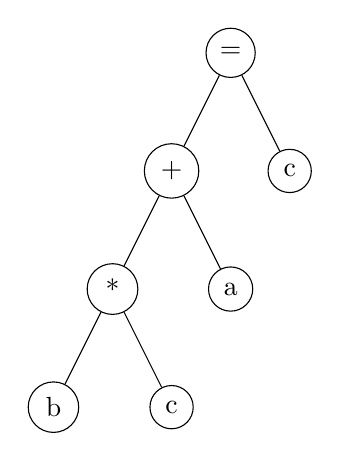
\begin{tikzpicture}
		    \tikzstyle{every node}=[circle,draw]
		    \node {=}
		        child {
		            node {+}
		            child { 	
		            			node {*} 
		            		 	child {node{b}}
			                    child {node{c}}
		            }
		            child { node {a} }
		        }
		        child { node {c} }
		    ;
		\end{tikzpicture}
	}
\end{center}

\newpage
\subsection{Verification des types}

La verification des types permet de controler la cohérence du langage d'entrée. Celle-ci est réalisée grâce à un parcours d'arbre couplé avec la table des symboles.
On commence par évaluer les types de chacunes des opérandes dans l'arbre puis on remonte ces types jusqu'aux opérateur afin de controler la compatibilité des opérandes dans l'expression. La verification des types renvoie le type de retour de l'expression, ou \verb?UNDEF? si la verification échoue.

\underline{Remarque : } On évalue en premier lieu, les sous-expression les plus en profondeur dans l'arbre syntaxique.
~~\\

\begin{algorithm}
\caption{checkType(tree, symTable) : Algorithme de verification des types}
\label{algo_verif_types}
\begin{algorithmic}
\REQUIRE $tree\ (syntaxic\_tree)$, $symTable (symbols\_table)$
\ENSURE $type\ (type\ de\ retour\ de\ l'expression\ ou_ UNDEF_ si_ l'expression\ est\ invalide)$
\IF {$tree.left.type == TYPE\_UNDEF$ or $tree.right.type == TYPE\_UNDEF$}
\RETURN $TYPE\_UNDEF$
\ENDIF	
\IF {$tree\_length(tree.left) < tree\_length(tree.right)$}
\STATE $ $
\ENDIF
\end{algorithmic}
\end{algorithm}

